%% LyX 2.0.6 created this file.  For more info, see http://www.lyx.org/.
%% Do not edit unless you really know what you are doing.
\documentclass[12pt,english,usenames,dvipsnames]{article}
\usepackage{amsthm}
\usepackage{amsmath}
\usepackage{fontspec}
\setmainfont[Mapping=tex-text]{Arial}
\setsansfont[Mapping=tex-text]{Arial}
\setmonofont{Arial Narrow}
\usepackage{listings}
\lstset{backgroundcolor={\color{shadebox}},
basicstyle={\small},
breaklines={true},
frame=single,
frameround=tttt,
framerule={.5pt},
morekeywords={GET,POST,PUT,DELETE},
otherkeywords={GET,POST,PUT,DELETE,HTTP/1.1, 200,OK,appication/xml},
stringstyle={\ttfamily},
tabsize=4}
\usepackage[letterpaper]{geometry}
\geometry{verbose,tmargin=1.8in,bmargin=1.25in,lmargin=1in,rmargin=1in}
\usepackage{fancyhdr}
\pagestyle{fancy}
\setcounter{secnumdepth}{5}
\setcounter{tocdepth}{5}
\setlength{\parskip}{\bigskipamount}
\setlength{\parindent}{0pt}
\usepackage{color}
\usepackage{array}
\usepackage{verbatim}
\usepackage{longtable}
\usepackage{multirow}
\usepackage{graphicx}

\makeatletter

%%%%%%%%%%%%%%%%%%%%%%%%%%%%%% LyX specific LaTeX commands.
%% Because html converters don't know tabularnewline
\providecommand{\tabularnewline}{\\}

%%%%%%%%%%%%%%%%%%%%%%%%%%%%%% Textclass specific LaTeX commands.

\numberwithin{equation}{section}
\numberwithin{figure}{section}
\usepackage{enumitem}		% customizable list environments
\newlength{\lyxlabelwidth}      % auxiliary length 
\numberwithin{table}{section}
\newenvironment{lyxcode}
{\par\begin{list}{}{
\setlength{\rightmargin}{\leftmargin}
\setlength{\listparindent}{0pt}% needed for AMS classes
\raggedright
\setlength{\itemsep}{0pt}
\setlength{\parsep}{0pt}
\normalfont\ttfamily}%
 \item[]}
{\end{list}}

%%%%%%%%%%%%%%%%%%%%%%%%%%%%%% User specified LaTeX commands.
\usepackage[usenames,dvipsnames,svgnames,table]{xcolor}
\usepackage{fancyhdr}
\usepackage{eso-pic}
\usepackage[stamp]{draftwatermark}
\usepackage{colortbl}

\SetWatermarkText{Draft 1.1.2l}
\SetWatermarkAngle{45}
\SetWatermarkLightness{0.9}
\SetWatermarkScale{.8}

\date{}
\lhead{\small{www.dedoimedo.com}}
\rhead{\small{some text}} 
\pagestyle{fancy}

\setlength{\headheight}{0.6in}
\setlength{\headwidth}{\textwidth}
\fancyhead[L]{}% empty left
\fancyhead[R]{ % right
   \includegraphics[height=0.75in]{../common/att_logo.png}
}
\pagestyle{fancy}

\definecolor{blue}{RGB}{79,129,189}
\definecolor{shadebox}{RGB}{255,255,204}

\cfoot{\scriptsize © 2014 AT\&T Intellectual Property. All rights reserved. AT\&T and AT\&T logo are trademarks of AT\&T Intellectual Property.}

\newcommand{\attcategory}[1]{\textbf{\Large Category: \textcolor{blue}{#1}}}
\newcommand{\attservice}[1]{\textbf{\Large Service:  \textcolor{blue}{#1}}}
\newcommand{\attdocumentnumber}[1]{\textbf{\small Document Number: #1}}
\newcommand{\attrevision}[1]{\textbf{\small Revision: #1}}
\newcommand{\attrevisiondate}[1]{\textbf{\small Revision Date: #1}}
\newcommand{\attauthor}[1]{\textbf{\small Author: #1}}


\let\oldtabular=\tabular
\def\tabular{\footnotesize\oldtabular}

\makeatother

\usepackage{xunicode}
\usepackage{polyglossia}
\setdefaultlanguage{english}
\begin{document}

\subsubsection{Functional Behavior}

\begin{comment}
Describe the functional behavior provided by this operation. Also
add here any special considerations, assumptions, and dependencies
for this particular operation
\end{comment}


The Modify WebRTC Call method modifies the state of the call through
session description protocol parameters. The following use cases are
able to be achieved using this method.
\begin{itemize}
\item Accept or Answer audio video calls.
\item Initiate : AudioVideo call Modifications.
\item Initiate : AudioVideo call Hold.
\item Initiate : AudioVideo call Resume.
\item Accept AudioVideo call Modifications.
\item Reject AudioVideo call\textbf{ }modifications .
\item Move call session to different device or endpoint (webRTC browser).
: First Step \{Put Call on Hold\}.
\item Call Transfer : The transferrer is a webRTC client and does have two
call session in open state which can be called as transferee and transfer-target.
This methodtriggers a communication between transferee and transfer.
\end{itemize}
\begin{comment}
Describe the functional behavior provided by this operation. Also
add here any special considerations, assumptions, and dependencies
for this particular operation
\end{comment}

The must set the following in order to use this method.
\begin{itemize}
\item The client must be registered and have a session ID allocated.
\item The client must maintain an event channel to be able to receive the
result of the AudioVideo call session modification invitation.
\item The client has AudioVideo call session with the state set to\textbf{
}session-open.
\end{itemize}
\begin{comment}
Describe the functional behavior provided by this operation. Also
add here any special considerations, assumptions, and dependencies
for this particular operation
\end{comment}



\subsubsection{Call flow - Ongoing Call Session}

\begin{comment}
Insert below a sequence diagram (ping pong) diagram in context to
a complete call flow or transaction with numbered arrows and some
description explaining the sequence as appropriate.
\end{comment}


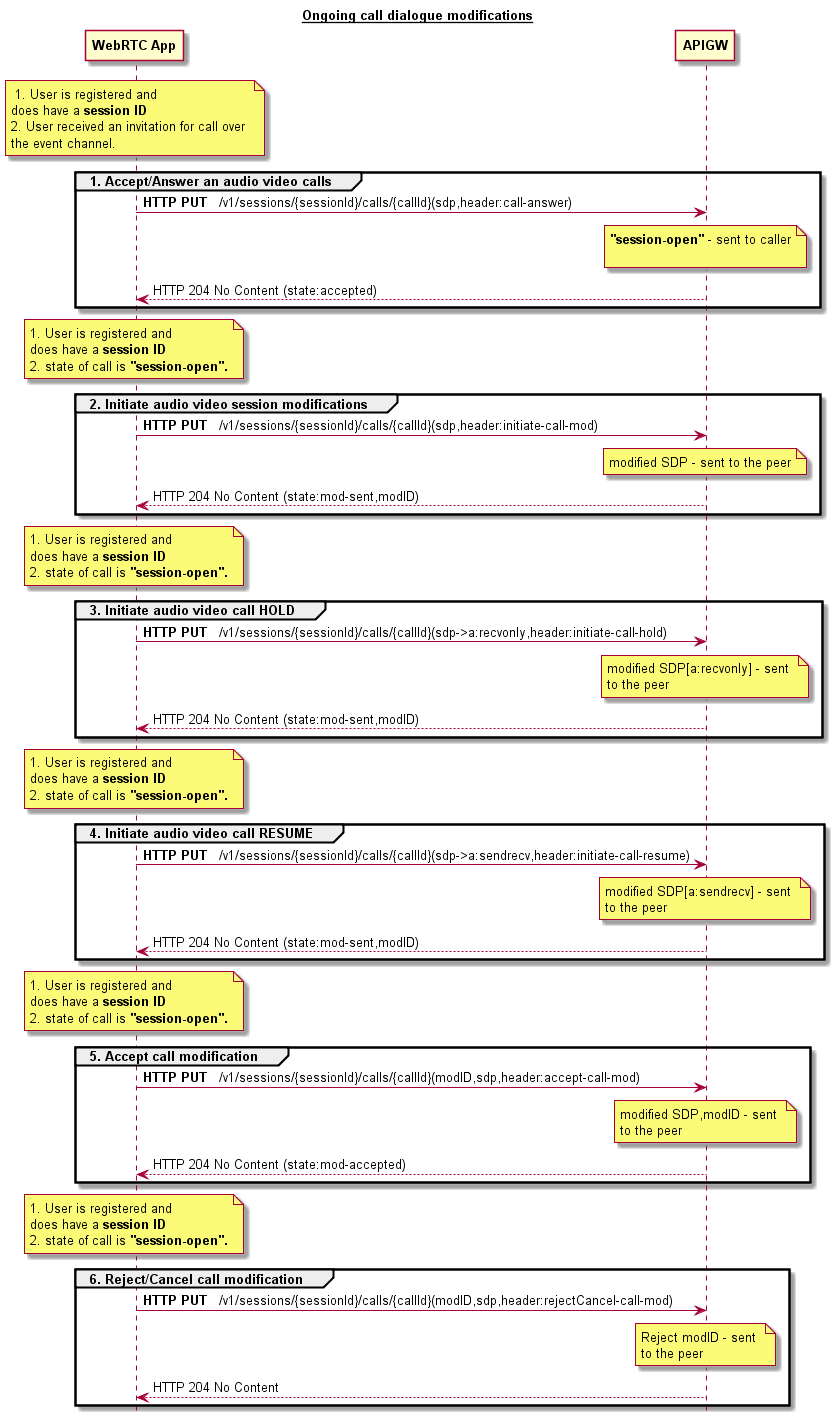
\includegraphics[scale=0.25]{sequence-diagram/modifyAudioVideoCalls}

\includegraphics[scale=0.2]{sequence-diagram/moveCall}

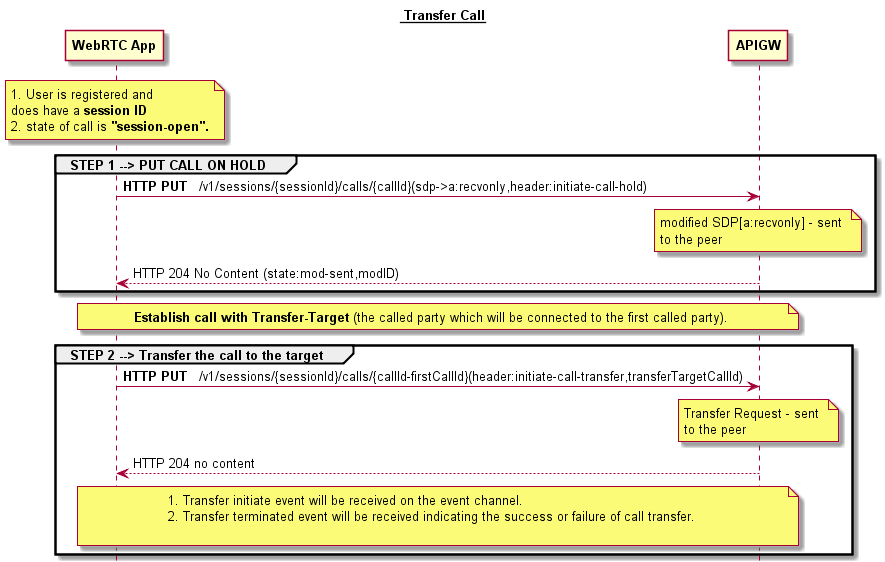
\includegraphics[scale=0.2]{sequence-diagram/TransferCall}


\subsubsection{Version Impact Summary}

\begin{comment}
Summarize the different versions of this operation that are in production
or deleted by the current release of this service. 
\end{comment}


\begin{longtable}{|>{\raggedright}p{0.15\textwidth}|>{\raggedright}p{0.16\textwidth}|>{\raggedright}p{0.55\textwidth}|}
\hline
\hline 
\textbf{\footnotesize{Service Version}} & \textbf{\footnotesize{Major or Minor Impact}} & \textbf{\footnotesize{Changes Introduced by this Version}}\tabularnewline
\hline 
\hline
\endfirsthead
\hline
\hline 
\textbf{\footnotesize{Service Version}} & \textbf{\footnotesize{Major or Minor Impact}} & \textbf{\footnotesize{Changes Introduced by this Version}}\tabularnewline
\hline 
\hline
\endhead
\hline 
{\footnotesize{1}} & {\footnotesize{Major}} & {\footnotesize{Initial Release}}\tabularnewline
\hline 
\end{longtable}


\subsubsection{Authentication and Authorization}

\begin{comment}
Describe OAuth model applicable to this operation.
\end{comment}


\begin{longtable}{|>{\raggedright}p{0.18\textwidth}|>{\raggedright}p{0.1\textwidth}|>{\raggedright}p{0.14\textwidth}|>{\raggedright}p{0.44\textwidth}|}
\hline
\hline 
\textbf{\footnotesize{Authorization Model}} & \textbf{\footnotesize{Subscriber Authorization required?}} & \textbf{\footnotesize{OAuth Scope Value}} & \textbf{\footnotesize{Brief Description}}\tabularnewline
\hline 
\hline
\endfirsthead
\hline
\hline 
\textbf{\footnotesize{Authorization Model}} & \textbf{\footnotesize{Subscriber Authorization required?}} & \textbf{\footnotesize{OAuth Scope Value}} & \textbf{\footnotesize{Brief Description}}\tabularnewline
\hline 
\hline
\endhead
\hline 
{\footnotesize{authorization\_code}} & {\footnotesize{Yes}} & WEBRTC & \begin{enumerate}
\item {\footnotesize{Redirect the user to AT\&T authorization page to capture
user consent.}}{\footnotesize \par}
\item {\footnotesize{Obtain OAuth access token using the OAuth authorization
code issued by the API Gateway along with the App Key and App Secret
by making a Get Access Token request with GrantType=authorization\_code.}}{\footnotesize \par}

\begin{enumerate}
\item Supports ICMN case
\end{enumerate}
\end{enumerate}


\tabularnewline
\hline 
{\footnotesize{client\_credentials}} & {\footnotesize{No}} & WEBRTC & \begin{enumerate}
\item {\footnotesize{Obtain OAuth access token with the App Key and App
Secret by making a Get Access Token request. }}{\footnotesize \par}

\begin{enumerate}
\item Supports VTN case 
\item Supports no-TN case {\footnotesize \par}
\end{enumerate}
\end{enumerate}


\tabularnewline
\hline 
\end{longtable}


\subsubsection{Representation Formats}

\begin{comment}
In the table below, describe supported representation formats for
the request and response body. Where different versions support different
formats, provide separate tables and indicate which versions apply
to each table. 
\end{comment}


\begin{longtable}{|>{\raggedright}p{0.16\textwidth}|>{\raggedright}p{0.7\textwidth}|}
\hline
\hline 
\textbf{\footnotesize{Direction}} & \textbf{\footnotesize{Supported Respresentation Formats}}\tabularnewline
\hline 
\hline
\endfirsthead
\hline
\hline 
\textbf{\footnotesize{Direction}} & \textbf{\footnotesize{Supported Respresentation Formats}}\tabularnewline
\hline 
\hline
\endhead
\hline 
{\footnotesize{Request}} & {\footnotesize{XML, JSON, URLENCODED}}\tabularnewline
\hline 
{\footnotesize{Response}} & {\footnotesize{XML, JSON, URLENCODED}}\tabularnewline
\hline 
\end{longtable}




\subsubsection{Input Parameters}

\begin{comment}
In the table below, describe input parameters. Where different versions
support different input parameters, provide separate tables and indicate
which versions apply to each table. The allowed values for the Location
in Request column are: Header, Resource URI, Body or Query Parameter.
\end{comment}


{\footnotesize{{\footnotesize{}}%
\begin{longtable}{|>{\raggedright}p{0.18\textwidth}|>{\raggedright}p{0.08\textwidth}|>{\raggedright}p{0.09\textwidth}|>{\raggedright}p{0.4\textwidth}|>{\raggedright}p{0.11\textwidth}|}
\hline
\hline 
\textbf{\footnotesize{Parameter }} & \textbf{\footnotesize{Data Type}} & \textbf{\footnotesize{Required?}} & \textbf{\footnotesize{Brief description}} & \textbf{\footnotesize{Location}}\tabularnewline
\hline 
\hline
\endfirsthead
\hline
\hline 
\textbf{\footnotesize{Parameter }} & \textbf{\footnotesize{Data Type}} & \textbf{\footnotesize{Required?}} & \textbf{\footnotesize{Brief description}} & \textbf{\footnotesize{Location}}\tabularnewline
\hline 
\hline
\endhead
\hline 
{\footnotesize{accept}} & {\footnotesize{String}} & {\footnotesize{No}} & {\footnotesize{Specifies the format of the body of the response. The
acceptable values for this parameter are:}}{\footnotesize \par}
\begin{itemize}
\item {\footnotesize{application/json}}{\footnotesize \par}
\item {\footnotesize{application/xml}}{\footnotesize \par}
\item {\footnotesize{application/x-www-form-urlencoded}}{\footnotesize \par}
\end{itemize}
{\footnotesize{The default value is application/json. }}{\footnotesize \par}

{\footnotesize{Per rfc2616: \textquotedbl{}If no Accept header field
is present, then it is assumed that the client accepts all media types.\textquotedbl{}
By default our services return application/json.}}{\footnotesize \par}

{\footnotesize{The normal Accept header processing rules shall be
followed according to rfc2616.}}{\footnotesize \par}

\emph{\footnotesize{Note}}{\footnotesize{: If there is no entity body
in a normal successful response, this parameter is still needed to
specify the format in the case of an error response message.}} & {\footnotesize{Header}}\tabularnewline
\hline 
{\footnotesize{authorization}} & {\footnotesize{String}} & {\footnotesize{Yes}} & {\footnotesize{Specifies the authorization type and token. The acceptable
format for this parameter is the phrase \textquotedbl{}Bearer OAuth
Token\textquotedbl{} followed by a space ( ) and an OAuth access token.
If this parameter value is missing from the header, then the API Gateway
returns a message with an HTTP status code of 400 Invalid Request.
If the OAuth access token is not valid, then the API Gateway returns
an HTTP status code of 401 Unauthorized with a WWW-Authenticate HTTP
header.}} & {\footnotesize{Header}}\tabularnewline
\hline 
{\footnotesize{x-calls-action}} & {\footnotesize{String}} & {\footnotesize{Yes}} & {\footnotesize{Specifies the action for a conference session . The
acceptable values for this parameter are:}}{\footnotesize \par}
\begin{itemize}
\item {\footnotesize{call-answer : The client accepts the call invitation.}}{\footnotesize \par}
\item {\footnotesize{initiate-call-mod : The client request for change in
media attributes, for example remove a video stream from an ongoing
call session.}}{\footnotesize \par}
\item {\footnotesize{initiate-call-hold : The Client request to put the
media path in a hold state.}}{\footnotesize \par}
\item {\footnotesize{initiate-call-transfer : The client put the call in
a hold state, calls another number, and bridges the two parties. }}{\footnotesize \par}
\item {\footnotesize{initiate-call-resume : The Client request to resume
the media path which was in a hold state.}}{\footnotesize \par}
\item {\footnotesize{initiate-call-move : The Client requests to move the
call to different registered active endpoint. }}{\footnotesize \par}
\item {\footnotesize{accept-call-mod : The client accepts the changes in
media attributes, for example remove a video stream from an ongoing
conference session.}}{\footnotesize \par}
\item {\footnotesize{rejectCancel-call-mod : The proposal from the remote
client to reject a media modification in an AudioVideo mod-received
event or the Initiate WebRTC Session request from the local client
to cancel a media modification.}}\end{itemize}
 & {\footnotesize{Header}}\tabularnewline
\hline 
{\footnotesize{x-transferTargetCallId}} & {\footnotesize{String}} & {\footnotesize{Yes}} & {\footnotesize{Specifies the call identifier of the transfer target.}} & {\footnotesize{Header}}\tabularnewline
\hline 
{\footnotesize{x-modId}} & {\footnotesize{String}} & {\footnotesize{Conditional}} & {\footnotesize{Specifies the modification identifier for media changes.}}{\footnotesize \par}

{\footnotesize{This parameter is required if the x-calls-action parameter
is set to accept-call-mod or rejectCancel-call-mod.}} & {\footnotesize{Header}}\tabularnewline
\hline 
{\footnotesize{x-reject-reason}} & {\footnotesize{String}} & {\footnotesize{No}} & {\footnotesize{Specifies the reason for rejecting the session media
changes.}}{\footnotesize \par}

{\footnotesize{This parameter is only applicable if the x-calls-action
parameter is set to rejectCancel-call-mod.}} & {\footnotesize{Header}}\tabularnewline
\hline 
{\footnotesize{callsMediaModifications}} & \multirow{1}{0.08\textwidth}{{\footnotesize{callsMediaModifications Object}}} & {\footnotesize{Yes}} & {\footnotesize{Contains the call media information.}} & {\footnotesize{Body}}\tabularnewline
\hline 
\end{longtable}{\footnotesize \par}

{\footnotesize{}}{\footnotesize \par}

\textbf{\footnotesize{Structure of callsMediaModifications Object}}{\footnotesize \par}

{\footnotesize{}}%
\begin{tabular}{|c|c|c|>{\centering}p{0.4\textwidth}|}
\hline 
\textbf{\footnotesize{Parameter}} & \textbf{\footnotesize{Data Type}} & \textbf{\footnotesize{Required?}} & \textbf{\footnotesize{Brief description}}\tabularnewline
\hline 
\hline 
{\footnotesize{sdp}} & {\footnotesize{Sdp Object}} & {\footnotesize{Yes}} & {\small{Contains an SDP offer for the audio video session.}}\tabularnewline
\hline 
\end{tabular}{\footnotesize \par}

\textbf{\footnotesize{Structure of sdp Object}}{\footnotesize \par}

{\footnotesize{}}%
\begin{longtable}{|c||c||c||>{\raggedright}p{0.4\textwidth}|}
\hline 
\textbf{\footnotesize{Parameter}} & \textbf{\footnotesize{Data Type}} & \textbf{\footnotesize{Required?}} & \textbf{\footnotesize{Brief description}}\tabularnewline
\hline 
\hline 
{\footnotesize{m}} & {\footnotesize{String}} & {\footnotesize{Yes}} & {\small{Specifies the media description in the following format.}}{\small \par}

{\small{m=<media> <port> <proto> <fmt>}}{\small \par}

{\small{The <media> field is the media type. }}{\footnotesize{The
only acceptable values for this field is:}}{\footnotesize \par}
\begin{itemize}
\item {\small{audio}}{\small \par}
\end{itemize}
{\small{The <port> field is the transport port to which the media
stream is sent.}}{\small \par}

{\small{<proto> is the transport protocol. }}{\footnotesize{The only
acceptable values for this field is:}}{\footnotesize \par}
\begin{itemize}
\item {\small{TCP/RTMP}}{\small \par}
\end{itemize}
{\small{The <fmt> field is a media format description.}}{\small \par}

{\small{The fourth and any subsequent sub-fields describe the format
of the media. The interpretation of the media format depends on the
value of the <proto> sub-field.}}\tabularnewline
\hline 
\hline 
{\footnotesize{attributes}} & {\footnotesize{List of Strings}} & {\footnotesize{Yes}} & {\small{Contains the attributes for extending SDP. This parameter
may be defined to be used as session-level attributes, media-level
attributes, or both.}}{\small \par}

{\small{The attribute fields may be in one of the following formats.}}{\small \par}

{\small{A property attribute is simply of the form:}}{\small \par}
\begin{itemize}
\item {\small{a=<flag> }}{\small \par}
\item {\small{These are binary attributes, and the presence of the attribute
conveys that the attribute is a property of the session. Example:
a=recvonly}}{\small \par}
\end{itemize}
{\small{A value attribute is of the form:}}{\small \par}
\begin{itemize}
\item {\small{a=<attribute>:<value>}}\end{itemize}
\tabularnewline
\hline 
\end{longtable}
}}{\footnotesize \par}

\pagebreak{}


\paragraph{Request – Example (Accept/Answer audioVideo Calls ) - JSON}

\begin{lstlisting}[backgroundcolor={\color{shadebox}},basicstyle={\footnotesize\ttfamily},frame=single,framerule={.5pt}]

PUT /RTC/v1/sessions/0045-ab42-89a2/calls/1234 HTTP/1.1
Content-Type: application/json;charset=UTF-8
Accept: application/json
x-calls-action: call-answer
Content-Length: xxx

{
    "callsMediaModifications": {
        "sdp": [
            {
                "m": "audio 9 TCP/RTMP 8",
                "attributes": [
                    {
                        "a": "sendrecv"
                    },
                    {
                        "a": "rtpmap:8 pcmu/8000/1"
                    },
                    {
                        "a": "setup:active"
                    }
                ]
            }
        ]
    }
}
\end{lstlisting}


\pagebreak{}


\paragraph{Request – Example (Accept/Answer audioVideo Calls ) - XML}

\begin{lstlisting}[backgroundcolor={\color{shadebox}},basicstyle={\footnotesize\ttfamily},frame=single,framerule={.5pt}]
PUT /RTC/v1/sessions/0045-ab42-89a2/calls/1234 HTTP/1.1
Content-Type: application/json;charset=UTF-8
Accept: application/xml
x-calls-action:call-answer
Content-Length: yyy

<?xml version="1.0" encoding="UTF-8" ?>
	<callsMediaModifications>
		<sdp>
			<m>audio 9 TCP/RTMP 8</m>
			<attributes>
				<a>sendrecv</a>
			</attributes>
			<attributes>
				<a>rtpmap:8 pcmu/8000/1</a>
			</attributes>
			<attributes>
				<a>setup:active</a>
			</attributes>
		</sdp>
	</callsMediaModifications>
\end{lstlisting}


\pagebreak{}


\paragraph{Request – Example (initiate audio video call session modifications
) - JSON}

\begin{lstlisting}[backgroundcolor={\color{shadebox}},basicstyle={\footnotesize\ttfamily},frame=single,framerule={.5pt}]

PUT /RTC/v1/sessions/0045-ab42-89a2/calls/1234 HTTP/1.1
Content-Type: application/json;charset=UTF-8
Accept: application/json
x-calls-action: initiate-call-mod
Content-Length: xxx

{
  "callsMediaModifications": {
    "sdp": [
      {
        "m": "audio 9000 RTP/AVP 8",
        "attributes": [
          { "a": "rcvonly" },
          { "a": "rtpmap:8 pcmu/8000/1" }
        ]
      },
      {
        "m": "video 9001 RTP/AVP 98",
        "attributes": [
          { "a": "rcvonly" },
          { "a": "rtpmap:98 H264/90000" },
          { "a": "fmtp:98 profile-levelid= A1438;packetization-mode=1" }
        ]
      }
    ]
  }
}

\end{lstlisting}


\pagebreak{}


\paragraph{Request – Example (initiate audio video call session modifications
) - XML}

\begin{lstlisting}[backgroundcolor={\color{shadebox}},basicstyle={\footnotesize\ttfamily},frame=single,framerule={.5pt}]

PUT /RTC/v1/sessions/0045-ab42-89a2/calls/1234 HTTP/1.1
Content-Type: application/xml;charset=UTF-8
Accept: application/xml
x-calls-action: initiate-call-mod
Content-Length: xxx

<?xml version="1.0" encoding="UTF-8" ?>
	<callsMediaModifications>
		<sdp>
			<m>audio 9000 RTP/AVP 8</m>
			<attributes>
				<a>rcvonly</a>
			</attributes>
			<attributes>
				<a>rtpmap:8 pcmu/8000/1</a>
			</attributes>
		</sdp>
		<sdp>
			<m>video 9001 RTP/AVP 98</m>
			<attributes>
				<a>rcvonly</a>
			</attributes>
			<attributes>
				<a>rtpmap:98 H264/90000</a>
			</attributes>
			<attributes>
				<a>fmtp:98 profile-levelid= A1438;packetization-mode=1</a>
			</attributes>
		</sdp>
	</callsMediaModifications>
	

\end{lstlisting}


\pagebreak{}


\paragraph{Request – Example (initiate audio video call hold ) - JSON}

\begin{lstlisting}[backgroundcolor={\color{shadebox}},basicstyle={\footnotesize\ttfamily},frame=single,framerule={.5pt}]

PUT /RTC/v1/sessions/0045-ab42-89a2/calls/1234 HTTP/1.1
Content-Type: application/json;charset=UTF-8
Accept: application/json
x-calls-action: initiate-call-hold
Content-Length: xxx

{
    "callsMediaModifications": {
        "sdp": [
            {
                "m": "audio 9 TCP/RTMP 8",
                "attributes": [
                    {
                        "a": "recvonly"
                    },
                    {
                        "a": "rtpmap:8 pcmu/8000/1"
                    }
                ]
            }
        ]
    }
}
\end{lstlisting}


\pagebreak{}


\paragraph{Request – Example (initiate audio video call hold ) - XML}

\begin{lstlisting}[backgroundcolor={\color{shadebox}},basicstyle={\footnotesize\ttfamily},frame=single,framerule={.5pt}]
PUT /RTC/v1/sessions/0045-ab42-89a2/calls/1234 HTTP/1.1
Content-Type: application/xml;charset=UTF-8
Accept: application/xml
x-calls-action: initiate-call-hold
Content-Length: xxx

<?xml version="1.0" encoding="UTF-8" ?>
	<callsMediaModifications>
		<sdp>
			<m>audio 9 TCP/RTMP 8</m>
			<attributes>
				<a>recvonly</a>
			</attributes>
			<attributes>
				<a>rtpmap:8 pcmu/8000/1</a>
			</attributes>
		</sdp>
	</callsMediaModifications>

\end{lstlisting}


\pagebreak{}


\paragraph{Request – Example (initiate audio video call resume ) - JSON}

\begin{lstlisting}[backgroundcolor={\color{shadebox}},basicstyle={\footnotesize\ttfamily},frame=single,framerule={.5pt}]

PUT /RTC/v1/sessions/0045-ab42-89a2/calls/1234 HTTP/1.1
Content-Type: application/json;charset=UTF-8
Accept: application/json
x-calls-action: initiate-call-resume
Content-Length: xxx

{
    "callsMediaModifications": {
        "sdp": [
            {
                "m": "audio 9 TCP/RTMP 8",
                "attributes": [
                    {
                        "a": "sendrecv"
                    },
                    {
                        "a": "rtpmap:8 pcmu/8000/1"
                    }
                ]
            }
        ]
    }
}
\end{lstlisting}


\pagebreak{}


\paragraph{Request – Example (initiate audio video call resume ) - XML}

\begin{lstlisting}[backgroundcolor={\color{shadebox}},basicstyle={\footnotesize\ttfamily},frame=single,framerule={.5pt}]

PUT /RTC/v1/sessions/0045-ab42-89a2/calls/1234 HTTP/1.1
Content-Type: application/xml;charset=UTF-8
Accept: application/xml
x-calls-action: initiate-call-resume
Content-Length: xxx

<?xml version="1.0" encoding="UTF-8" ?>
	<callsMediaModifications>
		<sdp>
			<m>audio 9 TCP/RTMP 8</m>
			<attributes>
				<a>sendrecv</a>
			</attributes>
			<attributes>
				<a>rtpmap:8 pcmu/8000/1</a>
			</attributes>
		</sdp>
	</callsMediaModifications>
\end{lstlisting}


\pagebreak{}


\paragraph{Request – Example (Accept audio video Media modifications ) - JSON}

\begin{lstlisting}[backgroundcolor={\color{shadebox}},basicstyle={\footnotesize\ttfamily},frame=single,framerule={.5pt}]


PUT /RTC/v1/sessions/0045-ab42-89a2/calls/1234 HTTP/1.1
Content-Type: application/json;charset=UTF-8
Accept: application/json
x-calls-action: accept-call-mod
x-modId:15011
Content-Length: xxx

{
  "callsMediaModifications": {
    "sdp": [
      {
        "m": "audio 9000 RTP/AVP 8",
        "attributes": [
          { "a": "rcvonly" },
          { "a": "rtpmap:8 pcmu/8000/1" }
        ]
      },
      {
        "m": "video 9001 RTP/AVP 98",
        "attributes": [
          { "a": "rcvonly" },
          { "a": "rtpmap:98 H264/90000" },
          { "a": "fmtp:98 profile-levelid= A1438;packetization-mode=1" }
        ]
      }
    ]
  }
}
\end{lstlisting}


\pagebreak{}


\paragraph{Request – Example (Accept audio video Media modifications ) - XML}

\begin{lstlisting}[backgroundcolor={\color{shadebox}},basicstyle={\footnotesize\ttfamily},frame=single,framerule={.5pt}]
PUT /RTC/v1/sessions/0045-ab42-89a2/calls/1234 HTTP/1.1
Content-Type: application/xml;charset=UTF-8
Accept: application/xml
x-calls-action: accept-call-mod
x-modId:15011
Content-Length: xxx

<?xml version="1.0" encoding="UTF-8" ?>
	<callsMediaModifications>
		<sdp>
			<m>audio 9000 RTP/AVP 8</m>
			<attributes>
				<a>rcvonly</a>
			</attributes>
			<attributes>
				<a>rtpmap:8 pcmu/8000/1</a>
			</attributes>
		</sdp>
		<sdp>
			<m>video 9001 RTP/AVP 98</m>
			<attributes>
				<a>rcvonly</a>
			</attributes>
			<attributes>
				<a>rtpmap:98 H264/90000</a>
			</attributes>
			<attributes>
				<a>fmtp:98 profile-levelid= A1438;packetization-mode=1</a>
			</attributes>
		</sdp>
	</callsMediaModifications>
\end{lstlisting}


\pagebreak{}


\paragraph{Request – Example (Reject/Cancel audio video Media modifications
) - JSON}

\begin{lstlisting}[backgroundcolor={\color{shadebox}},basicstyle={\footnotesize\ttfamily},frame=single,framerule={.5pt}]

PUT /RTC/v1/sessions/0045-ab42-89a2/calls/1234 HTTP/1.1
Content-Type: application/json;charset=UTF-8
Accept: application/json
x-calls-action: rejectCancel-call-mod
x-modId:15011
Content-Length: xxx

{
  "callsMediaModifications": {
    "sdp": [
      {
        "m": "audio 9000 RTP/AVP 8",
        "attributes": [
          { "a": "rcvonly" },
          { "a": "rtpmap:8 pcmu/8000/1" }
        ]
      },
      {
        "m": "video 9001 RTP/AVP 98",
        "attributes": [
          { "a": "rcvonly" },
          { "a": "rtpmap:98 H264/90000" },
          { "a": "fmtp:98 profile-levelid= A1438;packetization-mode=1" }
        ]
      }
    ]
  }
}
\end{lstlisting}


\pagebreak{}


\paragraph{Request – Example (Reject/Cancel audio video Media modifications)
- XML}

\begin{lstlisting}[backgroundcolor={\color{shadebox}},basicstyle={\footnotesize\ttfamily},frame=single,framerule={.5pt}]

PUT /RTC/v1/sessions/0045-ab42-89a2/calls/1234 HTTP/1.1
Content-Type: application/xml;charset=UTF-8
Accept: application/xml
x-calls-action: rejectCancel-call-mod
x-modId:15011
Content-Length: xxx

<?xml version="1.0" encoding="UTF-8" ?>
	<callsMediaModifications>
		<sdp>
			<m>audio 9000 RTP/AVP 8</m>
			<attributes>
				<a>rcvonly</a>
			</attributes>
			<attributes>
				<a>rtpmap:8 pcmu/8000/1</a>
			</attributes>
		</sdp>
		<sdp>
			<m>video 9001 RTP/AVP 98</m>
			<attributes>
				<a>rcvonly</a>
			</attributes>
			<attributes>
				<a>rtpmap:98 H264/90000</a>
			</attributes>
			<attributes>
				<a>fmtp:98 profile-levelid= A1438;packetization-mode=1</a>
			</attributes>
		</sdp>
	</callsMediaModifications>
\end{lstlisting}


\pagebreak{}


\paragraph{Request – Example (Transfer a call ) - JSON}

\begin{lstlisting}[backgroundcolor={\color{shadebox}},basicstyle={\footnotesize\ttfamily},frame=single,framerule={.5pt}]

PUT /RTC/v1/sessions/0045-ab42-89a2/calls/1234 HTTP/1.1
Content-Type: application/json;charset=UTF-8
Accept: application/json
x-calls-action: initiate-call-transfer
x-transferTargetCallId:1235
Content-Length: xxx

{
  "callsMediaModifications": {
    "sdp": [
      {
        "m": "audio 9000 RTP/AVP 8",
        "attributes": [
          { "a": "rcvonly" },
          { "a": "rtpmap:8 pcmu/8000/1" }
        ]
      },
      {
        "m": "video 9001 RTP/AVP 98",
        "attributes": [
          { "a": "rcvonly" },
          { "a": "rtpmap:98 H264/90000" },
          { "a": "fmtp:98 profile-levelid= A1438;packetization-mode=1" }
        ]
      }
    ]
  }
}
\end{lstlisting}


\pagebreak{}


\paragraph{Request – Example (Transfer a call) - XML}

\begin{lstlisting}[backgroundcolor={\color{shadebox}},basicstyle={\footnotesize\ttfamily},frame=single,framerule={.5pt}]

PUT /RTC/v1/sessions/0045-ab42-89a2/calls/1234 HTTP/1.1
Content-Type: application/xml;charset=UTF-8
Accept: application/xml
x-calls-action: initiate-call-transfer
x-transferTargetCallId:1235
Content-Length: xxx

<?xml version="1.0" encoding="UTF-8" ?>
	<callsMediaModifications>
		<sdp>
			<m>audio 9000 RTP/AVP 8</m>
			<attributes>
				<a>rcvonly</a>
			</attributes>
			<attributes>
				<a>rtpmap:8 pcmu/8000/1</a>
			</attributes>
		</sdp>
		<sdp>
			<m>video 9001 RTP/AVP 98</m>
			<attributes>
				<a>rcvonly</a>
			</attributes>
			<attributes>
				<a>rtpmap:98 H264/90000</a>
			</attributes>
			<attributes>
				<a>fmtp:98 profile-levelid= A1438;packetization-mode=1</a>
			</attributes>
		</sdp>
	</callsMediaModifications>
\end{lstlisting}


\pagebreak{}


\subsubsection{Output Parameters}

\begin{comment}
In the table below, describe output parameters. Where different versions
support different output parameters, provide separate tables and indicate
which versions apply to each table. Note: ‘consent’ refers to end
user consent which may need to be obtained before data is returned,
\end{comment}


{\footnotesize{{\footnotesize{}}%
\begin{longtable}{|>{\raggedright}p{0.18\textwidth}|>{\raggedright}p{0.08\textwidth}|>{\raggedright}p{0.09\textwidth}|>{\raggedright}p{0.4\textwidth}|>{\raggedright}p{0.11\textwidth}|}
\hline
\hline 
\textbf{\footnotesize{Parameter }} & \textbf{\footnotesize{Data Type}} & \textbf{\footnotesize{Required?}} & \textbf{\footnotesize{Brief description}} & \textbf{\footnotesize{Location}}\tabularnewline
\hline 
\hline
\endfirsthead
\hline
\hline 
\textbf{\footnotesize{Parameter }} & \textbf{\footnotesize{Data Type}} & \textbf{\footnotesize{Required?}} & \textbf{\footnotesize{Brief description}} & \textbf{\footnotesize{Location}}\tabularnewline
\hline 
\hline
\endhead
\hline 
x-modId & String & Conditional & Specifies the Identifier associated with the modification of media
attributes.

This parameter must be returned as a response to the initiation of
media modifications.

Note: This parameter is not applicable for a call session response

. & Header\tabularnewline
\hline 
x-state & String & Conditional & Specifies the state of the modifications request. & Header\tabularnewline
\hline 
\end{longtable}{\footnotesize \par}

{\footnotesize{}}
}}{\footnotesize \par}


\paragraph{Response – Example (Accept/Answer audioVideo Calls ) - JSON\protect \\
}

\texttt{}
\begin{lstlisting}[basicstyle={\footnotesize\ttfamily},tabsize=4]
HTTP/1.1 204 No Content
x-state: accepted
\end{lstlisting}



\paragraph{Response – Example (Accept/Answer audioVideo Calls ) - (XML)\protect \\
}

\begin{lstlisting}[basicstyle={\footnotesize\ttfamily}]
HTTP/1.1 204 No Content
x-state: accepted
\end{lstlisting}



\paragraph{Response – Example (initiate audio video call Media modifications
) - JSON\protect \\
}

\texttt{}
\begin{lstlisting}[basicstyle={\footnotesize\ttfamily},tabsize=4]
HTTP/1.1 204 No Content
x-modID: abc-1234-def-567
x-state: mod-sent
\end{lstlisting}



\paragraph{Response – Example (initiate audio video call session modifications
) - (XML)\protect \\
}

\begin{lstlisting}[basicstyle={\footnotesize\ttfamily}]
HTTP/1.1 204 No Content
x-modID: abc-1234-def-567
x-state: mod-sent
\end{lstlisting}



\paragraph{Response – Example (initiate audio video call hold ) - JSON\protect \\
}

\texttt{}
\begin{lstlisting}[basicstyle={\footnotesize\ttfamily},tabsize=4]
HTTP/1.1 204 No Content
x-modID: abc-1234-def-567
x-state: mod-sent
\end{lstlisting}



\paragraph{Response – Example (initiate audio video call hold ) - (XML)\protect \\
}

\begin{lstlisting}[basicstyle={\footnotesize\ttfamily}]
HTTP/1.1 204 No Content
x-modID: abc-1234-def-567
x-state: mod-sent
\end{lstlisting}



\paragraph{Response – Example (initiate audio video call resume ) - JSON\protect \\
}

\texttt{}
\begin{lstlisting}[basicstyle={\footnotesize\ttfamily},tabsize=4]
HTTP/1.1 204 No Content
x-modID: abc-1234-def-567
x-state: mod-sent
\end{lstlisting}



\paragraph{Response – Example (initiate audio video call resume ) - (XML)\protect \\
}

\begin{lstlisting}[basicstyle={\footnotesize\ttfamily}]
HTTP/1.1 204 No Content
x-modID: abc-1234-def-567
x-state: mod-sent
\end{lstlisting}



\paragraph{Response – Example (Accept audio video Media modifications ) - JSON\protect \\
}

\texttt{}
\begin{lstlisting}[basicstyle={\footnotesize\ttfamily},tabsize=4]
HTTP/1.1 204 No Content
x-modID: abc-1234-def-567
x-state: mod-accepted
\end{lstlisting}



\paragraph{Response – Example (Accept audio video Media modifications ) - (XML)\protect \\
}

\begin{lstlisting}[basicstyle={\footnotesize\ttfamily}]
HTTP/1.1 204 No Content
x-modID: abc-1234-def-567
x-state: mod-accepted
\end{lstlisting}



\paragraph{Response – Example (Reject/Cancel audio video Media modifications)
- JSON\protect \\
}

\texttt{}
\begin{lstlisting}[basicstyle={\footnotesize\ttfamily},tabsize=4]
HTTP/1.1 204 No Content
x-state: mod-rejectcancel
\end{lstlisting}



\paragraph{Response – Example (Reject/Cancel audio video Media modifications)
- (XML)\protect \\
}

\begin{lstlisting}[basicstyle={\footnotesize\ttfamily}]
HTTP/1.1 204 No Content
x-state: mod-sent
\end{lstlisting}



\subsubsection{HTTP Status Codes}

\begin{comment}
List expected response codes (indicate any variation that exists across
different versions):
\end{comment}


\begin{longtable}{|>{\raggedright}p{0.15\textwidth}|>{\raggedright}p{0.15\textwidth}|>{\raggedright}p{0.56\textwidth}|}
\hline
\hline 
\textbf{\footnotesize{Code}} & \textbf{\footnotesize{Reason Phrase}} & \textbf{\footnotesize{Description}}\tabularnewline
\hline 
{\footnotesize{200}} & {\footnotesize{OK}} & {\footnotesize{Successful response}}\tabularnewline
\hline
\endfirsthead
\hline
\hline 
\textbf{\footnotesize{Code}} & \textbf{\footnotesize{Reason Phrase}} & \textbf{\footnotesize{Description}}\tabularnewline
\hline 
{\footnotesize{200}} & {\footnotesize{OK}} & {\footnotesize{Successful response}}\tabularnewline
\hline
\endhead
\hline 
{\footnotesize{201}} & {\footnotesize{Created}} & {\footnotesize{Successful response and resource was successfully created.}}\tabularnewline
\hline 
{\footnotesize{202}} & {\footnotesize{Accepted}} & {\footnotesize{Successful response but action has not yet been enacted}}\tabularnewline
\hline 
{\footnotesize{204}} & {\footnotesize{No Content}} & {\footnotesize{Successful response and the response does not include
an entity.}}\tabularnewline
\hline 
{\footnotesize{206}} & {\footnotesize{Partial Content}} & {\footnotesize{The server has fulfilled the partial GET request for
the resource}}\tabularnewline
\hline 
{\footnotesize{304}} & {\footnotesize{Not Modified}} & {\footnotesize{Returned when the client has performed a conditional
GET request and access is allowed, but the resource has not been modified.}}\tabularnewline
\hline 
{\footnotesize{400}} & {\footnotesize{Bad Request}} & {\footnotesize{Many possible reasons not specified by the other codes.}}\tabularnewline
\hline 
{\footnotesize{401}} & {\footnotesize{Authentication Error}} & {\footnotesize{Authentication failed or was not provided.}}\tabularnewline
\hline 
{\footnotesize{403}} & {\footnotesize{Forbidden}} & {\footnotesize{Access permission error.}}\tabularnewline
\hline 
{\footnotesize{404}} & {\footnotesize{Not Found}} & {\footnotesize{The server has not found anything matching the Request-URI.
No indication is given of whether the condition is temporary or permanent.}}\tabularnewline
\hline 
{\footnotesize{405}} & {\footnotesize{Method Not Allowed}} & {\footnotesize{A request was made of a resource using a request method
not supported by that resource (e.g., using PUT on a REST resource
that only supports POST).}}\tabularnewline
\hline 
{\footnotesize{406}} & {\footnotesize{Not Acceptable}} & {\footnotesize{The resource identified by the request is only capable
of generating response entities which have content characteristics
not acceptable according to the accept headers sent in the request. }}\tabularnewline
\hline 
{\footnotesize{408}} & {\footnotesize{Request Timeout}} & {\footnotesize{The client did not produce a request within the time
that the server was prepared to wait. The client MAY repeat the request
without modifications at any later time. }}\tabularnewline
\hline 
{\footnotesize{409}} & {\footnotesize{Conflict}} & {\footnotesize{The request could not be completed due to a conflict
with the current state of the resource. This code is only allowed
in situations where it is expected that the user might be able to
resolve the conflict and resubmit the request. }}\tabularnewline
\hline 
{\footnotesize{411}} & {\footnotesize{Length Required}} & {\footnotesize{The Content-Length header was not specified.}}\tabularnewline
\hline 
{\footnotesize{413}} & {\footnotesize{Request Entity Too Large}} & {\footnotesize{The size of the request body exceed the maximum size
permitted.}}\tabularnewline
\hline 
{\footnotesize{414}} & {\footnotesize{Request-URI Too Long}} & {\footnotesize{The server is refusing to service the request because
the Request-URI is longer than the server is willing to interpret. }}\tabularnewline
\hline 
{\footnotesize{415}} & {\footnotesize{Unsupported Media Type}} & {\footnotesize{The request is in a format not supported by the requested
resource for the requested method.}}\tabularnewline
\hline 
{\footnotesize{500}} & {\footnotesize{Internal Server Error}} & {\footnotesize{The server encountered an internal error or timed out;
please retry.}}\tabularnewline
\hline 
{\footnotesize{503}} & {\footnotesize{Service Unavailable}} & {\footnotesize{The server is currently unable to receive requests;
please retry.}}\tabularnewline
\hline 
\end{longtable}


\subsubsection{Service Exceptions}

\begin{comment}
List the service exceptions generated by the operation (indicate any
variation that exists across different versions):
\end{comment}


\begin{longtable}{|>{\raggedright}p{0.1\textwidth}|>{\raggedright}p{0.33\textwidth}|>{\raggedright}p{0.33\textwidth}|>{\raggedright}p{0.1\textwidth}|}
\hline
\hline 
\textbf{\footnotesize{MessageId}} & \textbf{\footnotesize{Text}} & \textbf{\footnotesize{Variables}} & \textbf{\footnotesize{Parent HTTP Code}}\tabularnewline
\hline 
\hline
\endfirsthead
\hline
\hline 
\textbf{\footnotesize{MessageId}} & \textbf{\footnotesize{Text}} & \textbf{\footnotesize{Variables}} & \textbf{\footnotesize{Parent HTTP Code}}\tabularnewline
\hline 
\hline
\endhead
\hline 
{\footnotesize{SVC0001}} & {\footnotesize{A service error has occurred. Error code is <Error
Explanation>}} & {\footnotesize{Error Explanation : <content here>}} & {\footnotesize{400}}\tabularnewline
\hline 
{\footnotesize{SVC0002}} & {\footnotesize{Invalid input value for Message part <part name>}} & {\footnotesize{part name : name of the input parameter that resulted
in the error}} & {\footnotesize{400}}\tabularnewline
\hline 
{\footnotesize{SVC0003}} & {\footnotesize{Invalid input value for Message part <part name>, valid
values are <part values>}} & {\footnotesize{part value : value of input parameter that was found
to be in error.}} & {\footnotesize{400}}\tabularnewline
\hline 
{\footnotesize{SVC0004}} & {\footnotesize{No valid addresses provided in the Message part <part
name>}} & {\footnotesize{part name : name of the input parameter that resulted
in the error}} & {\footnotesize{400}}\tabularnewline
\hline 
\end{longtable}


\subsubsection{Policy Exceptions}

\begin{comment}
List the policy exceptions generated by the operation (indicate any
variation that exists across different versions):
\end{comment}


\begin{longtable}{|>{\raggedright}p{0.1\textwidth}|>{\raggedright}p{0.33\textwidth}|>{\raggedright}p{0.33\textwidth}|>{\raggedright}p{0.1\textwidth}|}
\hline
\hline 
\textbf{\footnotesize{MessageId}} & \textbf{\footnotesize{Text}} & \textbf{\footnotesize{Variables}} & \textbf{\footnotesize{Parent HTTP Code}}\tabularnewline
\hline 
\hline
\endfirsthead
\hline
\hline 
\textbf{\footnotesize{MessageId}} & \textbf{\footnotesize{Text}} & \textbf{\footnotesize{Variables}} & \textbf{\footnotesize{Parent HTTP Code}}\tabularnewline
\hline 
\hline
\endhead
\hline 
{\footnotesize{POL0001}} & {\footnotesize{A policy error occurred. For example, rate limit error,
authentication and authorization error.}} & {\footnotesize{N/A}} & {\footnotesize{401,403}}\tabularnewline
\hline 
{\footnotesize{POL0002}} & {\footnotesize{Privacy verification failed for address <address>,
request is refused}} & {\footnotesize{address : <content here>}} & {\footnotesize{403}}\tabularnewline
\hline 
{\footnotesize{POL0003}} & {\footnotesize{Too many addresses specified in Message part}} & {\footnotesize{N/A}} & {\footnotesize{403}}\tabularnewline
\hline 
{\footnotesize{POL1009}} & {\footnotesize{User has not been provisioned for \%1}} & {\footnotesize{System that hasn’t been provisioned}} & {\footnotesize{403}}\tabularnewline
\hline 
\end{longtable}
\end{document}
